% Created 2025-03-24 Mon 08:20
% Intended LaTeX compiler: lualatex
\documentclass[9qpt]{scrartcl}


\KOMAoptions{
%headings=chapterprefix,
twocolumn=true,
%toc=indenttextentries,
%toc=flat,
twoside=true,
headinclude=true,
footinclude=true
%  captions=topbeside
}
%\usepackage[fontsize=12.3]{scrextend}
\usepackage{fontspec}
\usepackage[T1]{fontenc}
\usepackage[english, portuguese]{babel}
\usepackage{hyperref}
%\usepackage[x11names,svgnames,table]{xcolor}
\usepackage[usenames,dvipsnames]{xcolor}
\defaultfontfeatures{Ligatures=TeX}
%%\setmainfont{Lato}
%%\setmainfont{Charis SIL}
\setmainfont{IBM Plex Serif}
\usepackage{typearea}
\usepackage{lscape}
\usepackage[a4paper]{geometry}
\geometry{a4paper,total={170mm,257mm},left=10mm,right=10mm, top=15mm, bottom=20mm}
\usepackage[english,portuguese]{babel}
\usepackage{amsmath,amsfonts,amsthm,bm}
\usepackage{graphicx}
\usepackage{float,wrapfig}
\usepackage{colortbl}
\usepackage{tabularx}
\usepackage{pst-labo}
\usepackage{setspace}
\usepackage{xfrac}
\usepackage{tikz}
\usepackage{pgfplots}
\pgfplotsset{compat=1.3}
%% Diagraman latex
\usepackage{endiagram}
\usepackage{smartdiagram}
\usepackage[tikz]{bclogo}
\usetikzlibrary{fit,patterns,shadows.blur,shapes,decorations.pathreplacing,decorations.markings,arrows.meta,arrows,positioning,shadows,trees}
\usetikzlibrary{decorations.pathmorphing} %% to chemfig config bond
\usepackage{upgreek}
\usepackage[modules={all}]{chemmacros}
%%\chemsetup{modules={reactions,spectroscopy,thermodynamics,redox,isotopes}}
%%\chemsetup{modules={all}}
\NewChemState\EPot{ symbol=E , subscript-pos=right , superscript=o, pre= , unit=\volt }
%\usepackage[version=4,arrows=pgf-filled]{mhchem}
\usepackage{chemfig,elements,cancel,siunitx}
\NewChemPhase\lqdd{\(\ell\)}
\NewChemPhase\gr{grafite}
\NewChemPhase\reac{reação}
%\setchemfig{fixed length=false, atom sep=2.0em, arrow offset=6pt, scheme debug=false,angle increment=30}
\setchemfig{angle increment=30, atom sep=1.67em, double bond sep=0.67ex, bond style={line width=0.1em}, cram width=0.8ex, cram dash width=0.1em, cram dash sep=0.2em, arrow style={line width=0.067em},  arrow head=-{Triangle}, arrow label sep=1ex, cycle radius coeff=0.75, chemfig style={line width=0.1em}, }
\renewcommand{\CancelColor}{\color{red}}
\usepackage{circuitikz}
\usepackage{mol2chemfig}
\usepackage{subfig,caption}
\captionsetup{font=small, labelfont={bf,sf}}
\usepackage{wrapfig,qrcode}
\usepackage{array,longtable} % ajust colunm table
\newcolumntype{J}{>{\centering\arraybackslash}m{7.5cm}}
\newcolumntype{K}{>{\centering\arraybackslash}m{6.5cm}}
\newcolumntype{L}{>{\centering\arraybackslash}m{5cm}}
\newcolumntype{B}{>{\centering\arraybackslash}m{2.5cm}}
\newcolumntype{N}{>{\centering\arraybackslash}m{1.4cm}}
\usepackage[most]{tcolorbox}
\newcounter{mycounter}
%%% Colobor
%%% Example colorbox
\newtcolorbox{Box2}[2][]{
lower separated=false,
colback=white,
colframe=black,fonttitle=\bfseries,
colbacktitle=black,
coltitle=white,
enhanced, attach boxed title to top left={yshift=-0.1in,xshift=0.15in}, boxed title style={boxrule=0pt,colframe=white,}, title=#2,#1}
%%%%%%%% Cabecalho
\usepackage{framed,amsmath}
\newtcolorbox{mybox}[2][]{
enhanced,title=#2, fonttitle=\sffamily\small,
top=2pt,
bottom=1mm,
boxrule=0.4pt,
coltitle=black,
colback=white,
attach boxed title to top center={yshift=-\tcboxedtitleheight/2,
yshifttext=-\tcboxedtitleheight/2},
boxed title style={
colframe=white,
colback=white,
left=0.2pt,
right=0.2pt},
#1}
\usepackage{tabularray}
%%%%%%
\newtcolorbox{exercisebox}%
{enhanced,breakable,colback=white, colframe=green!15!white,colbacktitle=white!15!pink, coltitle=pink!50!black,left=0pt,right=0mm,top=3mm,bottom=3mm,pad at break=0pt,bottomrule at break=0pt,toprule at break=0pt,borderline={0mm}{0mm}{green!50!white,dashed}, attach boxed title to top center={yshift=-2mm},boxed title style={boxrule=0.4pt},title=Exercícios,}
\usepackage{eso-pic}
\usepackage{etoolbox}
\usepackage{enumitem}
\newcommand\circitem[1]{%
\tikz[baseline=(char.base)]{%https://tex.stackexchange.com/questions/204116/uniform-size-of-circles-around-enumitems
\node[circle,draw=gray, fill=gray!30,
minimum size=1.2em,inner sep=0] (char) {#1};}}
\newcommand\boxitem[1]{%
\tikz[baseline=(char.base)]{%https://tex.stackexchange.com/questions/204116/uniform-size-of-circles-around-enumitems
\node[fill=orange!30,
minimum size=1.2em,inner sep=0] (char) {#1};}}
%\usepackage{widetext}% needs packages "flushend" & "cuted" of "sttools" % bundle, which perhaps must separately be installed
\newcommand{\dd}[1]{\hspace{2pt}d#1}
\definecolor{color1}{RGB}{0,0,90} % Color of the article title and sections
\definecolor{color2}{RGB}{0,20,20} % Color of the boxes behind the abstract and
\definecolor{cinza}{HTML}{C0C0C0}
%%% Custom Exercios
\usepackage{bohr}
\usepackage{multicol}
\setlength{\columnsep}{1.5cm}
\setlength{\columnseprule}{0.2pt}
\usepackage[no-files]{xsim}
\usepackage{tasks}
\xsimsetup{
goal-print={\pgfmathprintnumber[fixed zerofill,precision=1]{#1}}
}
\newcommand*\circled[2]{\tikz[baseline=(char.base)]{
\node[shape=circle,fill,inner sep=2pt, text=white] (char) {#1};}}
%%%%%-Custom Xsim exercises %%%%%
\DeclareExerciseEnvironmentTemplate{custom}
{%\item[\GetExerciseProperty{counter}]
\Needspace*{0\baselineskip}
\noindent
\circled{\XSIMmixedcase{\GetExerciseProperty{counter}}}~~~%
\noindent
\IfInsideSolutionF{%
\GetExercisePropertyT{points}{ % notice the space
(%
\printgoal{\PropertyValue}
\IfExerciseGoalSingularTF{points}
{%\XSIMtranslate{point}
}
{% \XSIMtranslate{points}
}%
)%
}
}}
{\vspace{\baselineskip}}
%%%%%------- Custom  resposta -------%%%%%%%
\DeclareExerciseEnvironmentTemplate{space}
%{\textbf{\GetExerciseProperty{counter}} }
{\noindent\circled{\XSIMmixedcase{\GetExerciseProperty{counter}}}~~~}
% {\circled{\XSIMmixedcase{\GetExerciseProperty{counter}}}}~~~%
{\qquad}
\newcommand*\answer[1]{%
\XSIMexpandcode{%
\SetExerciseProperty{solution-body}
{\noexpand{\Alph{task}}}}%
#1%
}
%\sisetup{locale=DE}
\xsimsetup{
collect = true,
exercise/within = section,
exercise/template = custom,
exercise/the-counter =  \arabic{exercise},
solution/template= custom ,
%%solution-name = solution,  % used with headings=true
%solution/print=true,
%print-collection/print=both,
%print-solutions/collection=true
%goal-print= {\pgfmathprintnumber[fixed zerofill,precision=1]\num{#1}}
}
\RenewDocumentCommand\printpoints{}{%
\TotalExerciseTypeGoal{exercise}{points}{}{}%
}
\NewTasksEnvironment[label = (\emph{\alph*}), label-width = 12pt]{choice}[\choice]
\newenvironment{questions}{\itemize}{\enditemize}
\everymath{\displaystyle}
\DeclareExerciseHeadingTemplate{solution}{%
\section*{Gabarito}%
}
%\usepackage{filecontents}
\NewTblrTheme{fancy}{
\SetTblrStyle{firsthead}{font=\bfseries}
\SetTblrStyle{firstfoot}{fg=blue2}
\SetTblrStyle{middlefoot}{\itshape}
\SetTblrStyle{caption-tag}{red2}
}

\newcommand{\lh}{\underline{\hspace{1cm}}}
%%\onehalfspacing
\def\professor{Fábio Lima}
\def\aluno{ }
\def\numerochamada{}
\def\disciplina{Química}
%%\def\disciplina{UC III}
%%\def\disciplina{R.A.}
\def\turma{3 Ano }
%%\def\tipo{{\bfseries Avaliação Bimestral}}
\def\tipo{\bfseries Simulado }
%\def\tipo{\bfseries Atividade Avaliativa}
\def\bimestre{1 Bimestre}
%\def\escola{E.E. 26 de Agosto}
%\def\escola{E.E. José Mamede de Aquino}
\def\escola{E.E. Joaquim Murtinho}
\def\dataprova{}
\DeclareExerciseCollection{TeoriaAtomica}
\DeclareExerciseCollection{GeometriaMolecular}
\DeclareExerciseCollection{Polaridade}
\DeclareExerciseCollection{LigacaoQuimica}
\DeclareExerciseCollection{PilhasI}
\DeclareExerciseCollection{TermoquimicaI}
\date{\today}
\title{}
\hypersetup{
 pdfauthor={},
 pdftitle={},
 pdfkeywords={},
 pdfsubject={},
 pdfcreator={Emacs 30.1 (Org mode 9.7.11)}, 
 pdflang={English}}
\begin{document}

\selectlanguage{portuguese}
\twocolumn[
%\input{../Modelos/CabeOficial}
\input{../Modelos/cabenovo}
%\input{../Modelos/mamede}
%\input{../Modelos/26agosto}
%% \input{../Modelos/geral}
%Cada questão vale {\textbf 2,0}

%%\section*{Regime de Progressão Parcial}
%\section*{Atividade}
%\section*{Trabalho}
%%\section*{\disciplina}

%{\bfseries Obrigatório a resolução das questões }

%\input{../Modelos/gabarito}

%%Total Prova: \printpoints
\smallbreak
\medbreak
\par\vspace{2ex}]%%%%\input{../Modelos/mamede}


\collectexercises{TeoriaAtomica}

\begin{exercise}[points=1.0]
O átomo é a menor partícula que identifica um elemento químico. Ele possui duas partes, a saber: uma delas é o núcleo, constituído por prótons e nêutrons, e a outra é a região externa – a eletrosfera-, por onde circulam os elétrons. Alguns experimentos permitiram a descoberta das características das partículas constituintes do átomo.

Em relação a essas características, indique a alternativa correta.

\begin{choice}
\choice prótons e elétrons possuem massas iguais e cargas elétricas de sinais opostos.
\choice  entre as partículas atômicas, os elétrons têm maior massa e ocupam maior volume no átomo.
\choice entre as partículas atômicas, os prótons e os nêutrons têm maior massa e ocupam maior volume no átomo.
\choice entre as partículas atômicas, os prótons e os nêutrons têm mais massa, mas ocupam um volume muito pequeno em relação ao volume total do átomo.
\choice As partículas não possuem massa.
\end{choice}
\end{exercise}
\begin{solution}
LETRA D
\end{solution}


\begin{exercise}[points=1.0]
Os estudos realizados por Rutherford mostraram que o átomo deveria ser constituído por um núcleo positivo com elétrons girando ao seu redor. Os elétrons foram inicialmente levados em consideração no modelo atômico proposto pelo seguinte pesquisador.

\begin{choice}
\choice  Niels Borh
\choice J. J. Thomson
\choice John Dalton.
\choice  Werner Heisenberg
\choice Max Planck
\end{choice}
\end{exercise}
\begin{solution}
LETRA B
\end{solution}


\begin{exercise}[points=1.0]
Comemora-se, neste ano de 2011, o centenário do modelo atômico proposto pelo
físico neozelandês Ernest Rutherford (1871-1937), prêmio Nobel da Química em 1908. Em 1911,Rutherford, bombardeou uma finíssima lâmina de ouro com partículas alfa, oriundas de uma amostra contendo o elemento químico polônio. De acordo com o seu experimento, Rutherford concluiu que

\begin{choice}
\choice o átomo é uma partícula maciça e indestrutível.
\choice os elétrons estão mergulhados em uma massa homogênea de carga positiva.
\choice a maioria das partículas alfa sofria um desvio ao atravessar a lâmina de ouro.
\choice existem, no átomo, mais espaços vazios do que preenchidos.
\choice o átomo é pudim de passas incrustado de carga negativa em um esfera positiva
\end{choice}
\end{exercise}
\begin{solution}
LETRA C
\end{solution}



\begin{exercise}[points=1.0]
O filme \emph{"Homem de Ferro 2"} retrata a jornada de Tony Stark para substituir o metal paládio, que faz parte do reator de seu peito, por um metal atóxico. Após interpretar informações deixadas por seu pai, Tony projeta um holograma do potencial substituto, cuja imagem se assemelha à figura abaixo

\begin{center}
\tikzset{every picture/.style={line width=0.75pt}} %set default line width to 0.75pt        

\begin{tikzpicture}[x=0.75pt,y=0.75pt,yscale=-1,xscale=1]
%uncomment if require: \path (0,300); %set diagram left start at 0, and has height of 300

%Shape: Circle [id:dp5016060929568149] 
\draw   (108,184) .. controls (108,153.07) and (133.07,128) .. (164,128) .. controls (194.93,128) and (220,153.07) .. (220,184) .. controls (220,214.93) and (194.93,240) .. (164,240) .. controls (133.07,240) and (108,214.93) .. (108,184) -- cycle ;
%Shape: Circle [id:dp7913851496733558] 
\draw  [color={rgb, 255:red, 8; green, 8; blue, 8 }  ,draw opacity=1 ][fill={rgb, 255:red, 10; green, 10; blue, 10 }  ,fill opacity=1 ] (146.5,184) .. controls (146.5,174.34) and (154.34,166.5) .. (164,166.5) .. controls (173.66,166.5) and (181.5,174.34) .. (181.5,184) .. controls (181.5,193.66) and (173.66,201.5) .. (164,201.5) .. controls (154.34,201.5) and (146.5,193.66) .. (146.5,184) -- cycle ;
\end{tikzpicture}

\end{center}
\vspace{2cm}

Essa imagem é uma representação do modelo de
\begin{choice}
\choice Rutherford.
\choice Thomson.
\choice Dalton.
\choice Howard Stark  
\choice Frezza
\end{choice}
\end{exercise}
\begin{solution}
LETRA A
\end{solution}


\begin{exercise}[points=1.0]
Para o valor do número quântico principal \textbf{n} igual a 4, os tipos de orbitais que podem existir na configuração eletrônica de um átomo podem ser:
\begin{choice}
\choice  s, p, d, f.
\choice  somente s, p, d.
\choice  somente p e f.
\choice somente s e p.
\choice somente d e f
\end{choice}
\end{exercise}
\begin{solution}
LETRA A
\end{solution}



\begin{exercise}[points=1.0]
O bombardeamento da folha de ouro com partículas alfa, no experimento de Rutherford, mostra que algumas dessas partículas sofrem desvio acentuado do seu trajeto, o que é devido ao fato de que as partículas alfa:
\begin{choice}(1)
\choice Chocam-se com as moléculas de ouro.
\choice Têm carga negativa e são repelidas pelo núcleo.
\choice São muito lentas e qualquer obstáculo as desvia.
\choice Têm carga positiva e são repelidas pelo núcleo.
\choice Não podem atravessar a lâmina de ouro.
\end{choice}
\end{exercise}
\begin{solution}
LETRA D
\end{solution}



\begin{exercise}[points=1.0]
A experiência de Rutherford, que foi, na verdade, realizada por dois de seus orientados, Hans Geiger e Ernest Marsden, serviu para refutar especialmente o modelo atômico:
\begin{choice}(2)
\choice de Bohr.
\choice de Thomson.
\choice planetário.
\choice quântico.
\choice de Dalton.
\end{choice}
\end{exercise}
\begin{solution}
LETRA B
\end{solution}

\begin{exercise}[points=1.0]
Assinale a afirmativa que descreve ADEQUADAMENTE a teoria atômica de Dalton. Toda matéria é constituída de átomos:
\begin{choice}
\choice os quais são formados por partículas positivas e negativas.
\choice os quais são formados por um núcleo positivo e por elétrons que gravitam livremente em torno desse núcleo.
\choice os quais são formados por um núcleo positivo e por elétrons que gravitam em diferentes camadas eletrônicas.
\choice e todos os átomos de um mesmo elemento são idênticos.
\choice Nenhuma das alternativas acima.
\end{choice}
\end{exercise}
\begin{solution}
LETRA D
\end{solution}



\begin{exercise}[points=1.0]
Quem introduziu pela primeira vez o princípio da incerteza?

\begin{choice}(2)
\choice Pauli
\choice De Broglie
\choice Dirac
\choice Schrödinger
\choice Heisenberg
\end{choice}
\end{exercise}
\begin{solution}
Letra E
\end{solution}



\begin{exercise}[points=1.0]
Qual das alternativas a seguir \textbf{NÃO} é uma limitação do modelo de Bohr do átomo?

\begin{choice}
\choice Os elétrons se movem ao redor do núcleo em órbitas circulares e planas.
\choice Os elétrons são considerados apenas como partículas e não como ondas.
\choice É possível determinar com precisão a posição e o momento de um elétron simultaneamente.
\choice Os elétrons dentro dos átomos só podem ocupar níveis de energia quantizados.
\choice Ele explica apenas o espectro de emissão de linha do átomo de hidrogênio.
\end{choice}
\end{exercise}
\begin{solution}
C
\end{solution}



\begin{exercise}[points=1.0]
Qual das seguintes afirmações é \textbf{verdadeira} sobre um elétron?

\begin{choice}
\choice Está localizado mais longe do núcleo quando absorve energia.
\choice Absorve energia quando se move de um estado de maior energia para o estado fundamental.
\choice Está localizado no núcleo quando absorve energia.
\choice Está localizado mais perto do núcleo quando absorve energia.
\choice Quando libera energia se move para um estado de maior energia
\end{choice}
\end{exercise}
\begin{solution}
E
\end{solution}



\begin{exercise}[points=1.0]
Qual das alternativas a seguir melhor descreve um \textbf{elétron}?
\begin{choice}
\choice Uma partícula carregada positivamente com uma massa muito menor que a do núcleo
\choice Uma partícula carregada negativamente com uma massa muito menor que a do núcleo
\choice Uma partícula carregada positivamente com uma massa muito maior que a do núcleo
\choice Uma partícula carregada negativamente com uma massa muito maior que a do núcleo
\choice Partícula neutra com massa igual à do núcleo.
\end{choice}
\end{exercise}
\begin{solution}
D
\end{solution}



\begin{exercise}[points=1.0]
Qual das alternativas a seguir melhor define o \textbf{número atômico} ?

\begin{choice}
\choice O número total de prótons e nêutrons no núcleo de um átomo
\choice O número de prótons no núcleo de um átomo
\choice O número de nêutrons no núcleo de um átomo
\choice O número total de prótons, nêutrons e elétrons em um átomo
\choice O número de elétrons no núcleo de um átomo
\end{choice}
\end{exercise}
\begin{solution}
B
\end{solution}





\begin{exercise}[points=1.0]
Uma moda recente entre as crianças é colecionar figurinhas que brilham no escuro. As figuras apresentam em sua constituição, a substância sulfeto de zinco. O fenômeno ocorre porque alguns elétrons que compõem os átomos de zinco absorvem energia luminosa, saltando para níveis de energia mais externos. No escuro, esses elétrons retornam aos seus níveis de origem, liberando energia luminosa e fazendo a figurinha brilhar.

Essa característica pode ser explicada considerando o modelo atômico proposto por:

\begin{choice}
\choice Bohr.
\choice Rutherford.
\choice Lavoisier.
\choice Thomson.
\choice Dalton.
\end{choice}
\end{exercise}
\begin{solution}
A
\end{solution}



\begin{exercise}[points=1.0]
Qual das imagens a seguir representa melhor o modelo atômico do pudim de passas de Thomson?


\begin{choice}(1)
\choice \resizebox{.2\textwidth}{!}{%
\begin{circuitikz}
\tikzstyle{every node}=[font=\LARGE]
\draw  (2,12.25) circle (1.75cm);
\draw  (1,13.25) circle (0.25cm);
\draw  (2,13.25) circle (0.25cm);
\draw  (1.5,12) circle (0.25cm);
\draw  (2.75,12.25) circle (0.25cm);
\draw  (2.25,11.25) circle (0.25cm);
\node [font=\LARGE] at (1.5,11) {+};
\node [font=\LARGE] at (3,13) {+};
\node [font=\LARGE] at (2.5,11.5) {+};
\node [font=\LARGE] at (0.75,12.25) {+};
\node [font=\LARGE] at (2,12.5) {+};
\node [font=\LARGE] at (2.25,11.25) {-};
\node [font=\LARGE] at (2.75,12.25) {-};
\node [font=\LARGE] at (2,13.25) {-};
\node [font=\LARGE] at (1,13.25) {-};
\node [font=\LARGE] at (1.5,12) {-};
\end{circuitikz}
}%


\choice \resizebox{.2\textwidth}{!}{%
\begin{circuitikz}
\tikzstyle{every node}=[font=\LARGE]
\draw [fill={rgb, 255:red, 122; green, 119; blue, 119 }  ,fill opacity=1 ] (2,12.25) circle (1.75cm);
\end{circuitikz}
}%







\choice 	\resizebox{0.2\textwidth}{!}{%
		\begin{circuitikz}
			\tikzstyle{every node}=[font=\LARGE]
			\draw  (2,12.25) circle (1.75cm);
			\draw  (0.75,12.25) circle (0.25cm) node {\LARGE -} ;
			\draw  (1.5,13.25) circle (0.25cm);
			\draw  (3,12.5) circle (0.25cm);
			\draw  (2.25,11) circle (0.25cm) node {\LARGE -} ;
			\draw  (2,12.25) circle (0.5cm);
			\node [font=\huge] at (2,12.25) {+};
			\node [font=\large] at (1.5,13.25) {-};
			\node [font=\large] at (3,12.5) {-};
		\end{circuitikz}
	}%

\choice \resizebox{.2\textwidth}{!}{%
\begin{circuitikz}
\tikzstyle{every node}=[font=\LARGE]
\draw  (2,12.25) circle (1.75cm);
\draw [ fill={rgb,255:red,192; green,191; blue,188} ] (2,10.5) circle (0.25cm) node {\LARGE -} ;
\draw [ fill={rgb,255:red,192; green,191; blue,188} ] (0.25,12) circle (0.25cm) node {\LARGE -} ;
\draw [ fill={rgb,255:red,192; green,191; blue,188} ] (2,14) circle (0.25cm) node {\LARGE -} ;
\draw [ fill={rgb,255:red,192; green,191; blue,188} ] (3.75,12) circle (0.25cm) node {\LARGE -} ;
\draw  (2,12.25) circle (0.5cm) node {\LARGE +} ;
\end{circuitikz}
}%



\choice \resizebox{.2\textwidth}{!}{%
\begin{circuitikz}
\tikzstyle{every node}=[font=\LARGE]
\draw  (2,12.25) circle (1.75cm);
\draw  (2,12.25) circle (0.5cm) node {\LARGE +} ;
\end{circuitikz}
}%

\end{choice}
\end{exercise}




\begin{exercise}[points=1.0]
Qual químico descobriu que os elétrons existem em níveis de energia fixos?
\begin{choice}
\choice Bohr
\choice Thomson
\choice Dalton
\choice Geiger e Marsden
\choice Rutherford
\end{choice}
\end{exercise}
\begin{solution}
A
\end{solution}


\begin{exercise}[points=1.0]
Na experiência de Geiger-Marsden supervisionada por Ernest Rutherford (conhecida como a experiência da folha de ouro de Rutherford), que tipo de partícula foi dispersada por uma folha de ouro, provando que os átomos contêm um núcleo denso?

\begin{choice}
\choice Raios gama
\choice Nêutrons
\choice Partículas \(\upbeta^+\)
\choice Partículas \(\upbeta^-\)
\choice Partículas \(\upalpha\)
\end{choice}
\end{exercise}

\begin{solution}
E
\end{solution}

\begin{exercise}[points=1.0]
Qual é a principal força atrativa entre partículas no núcleo de um átomo?

\begin{choice}
\choice Gravidade
\choice Forca eletrostática
\choice Força nuclear forte
\choice Força nuclear fraca
\choice Força eletromagnética
\end{choice}
\end{exercise}
\begin{solution}
C
\end{solution}

\begin{exercise}[points=1.0]
Que passo em frente, a partir do modelo atômico das orbitais de Bohr, foi dado por Schrödinger no seu modelo da nuvem eletrónica?

\begin{choice}
\choice O núcleo contém partículas com massa mas sem carga.
\choice Os elétrons ocupam níveis de energia com raios fixos.
\choice O núcleo contém partículas com massa e carga positiva.
\choice Os elétrons movem-se dentro de uma esfera positivamente carregada.
\choice Os elétrons estão dispersos no espaço.
\end{choice}
\end{exercise}
\begin{solution}
E
\end{solution}


\begin{exercise}[points=1.0]
Em que é que o modelo atômico de Thomson é diferentes do modelo atômico de Dalton?

\begin{choice}
\choice O modelo atômico de Thomson inclui partículas com carga negativa conhecidas como elétrons
\choice O modelo atômico de Thomson mostra elétrons a ocupar os vértices de um cubo.
\choice O modelo atômico de Thomson inclui partículas com carga positiva conhecidas como prótons
\choice O modelo atômico de Thomson descreve elétrons a orbitar um núcleo central.
\choice O modelo atômico de Thomson mostra elétrons a ocupar diferentes níveis de energia.
\end{choice}
\end{exercise}
\begin{solution}
A
\end{solution}



\collectexercisesstop{TeoriaAtomica}
\collectexercises{GeometriaMolecular}


\begin{exercise}[points=1]
Qual é a geometria molecular da molécula de metano (\ch{CH4})?

\begin{choice}
\choice Linear
\choice Angular
\choice Tetraédrica
\choice Octaédrica
\choice Piramidal
\end{choice}
\end{exercise}


\begin{exercise}[points=1]
Quanto maior o número de átomos em uma molécula, maior a quantidade de geometrias moleculares possíveis No caso das moléculas triatômicas, elas podem apresentar geometria linear ou angular.

São exemplos de moléculas com pares de elétrons disponíveis no átomo central e que conferem a geometria angular da molécula, \textbf{EXCETO}:


\begin{choice}(2)
\choice \ch{H2S}
\choice \ch{CO2}
\choice \ch{SO2}
\choice \ch{H2O}
\choice \ch{N2}
\end{choice}
\end{exercise}


\begin{exercise}[points=1]
A molécula do \ch{OF2} é polar, e a molécula do \ch{BeF2} é não polar. Isto se deve à (ao):

\begin{choice}
\choice diferença de eletronegatividade entre os átomos nas respectivas moléculas
\choice  geometria molecular
\choice tamanho dos átomos ligados ao flúor.
\choice grande reatividade do oxigênio em relação ao flúor.
\choice fato de o oxigênio e o flúor serem gases.
\end{choice}
\end{exercise}




\begin{exercise}[points=1]
Assinale a opção que contém a geometria molecular CORRETA das espécies OF₂ , SF₂ , BF₃ , NF₃ , CF₄ e XeO₄ , todas no estado gasoso. 

\begin{choice}
\choice Angular, linear, piramidal, piramidal, tetraédrica e quadrado planar. 
\choice Linear, linear, trigonal plana, piramidal, quadrado planar e quadrado planar. 
\choice Angular, angular, trigonal plana, piramidal, tetraédrica e tetraédrica. 
\choice Linear, angular, piramidal, trigonal plana, angular e tetraédrica.
\choice Trigonal plana, linear, tetraédrica, piramidal, tetraédrica e quadrado planar.
\end{choice}
\end{exercise}
\begin{solution}
C
\end{solution}




\begin{exercise}
Assinale a opção que contém, respectivamente, a geometria das moléculas \ch{NH3} e \ch{SiC$\ell$4} no estado
gasoso:
\#+begin\textsubscript{chocie} 
\choice Plana; plana.
\choice Piramidal; plana.
\choice Plana; tetragonal.
\choice Piramidal; piramidal.
\choice Piramidal; tetragonal.
\#+end\textsubscript{choice}
\end{exercise}




\collectexercisesstop{GeometriaMolecular}



\collectexercises{Polaridade}

\begin{exercise}[points=1.0]
O aumento da diferença de eletronegatividade entre os elementos ocasiona a seguinte ordem no caráter das ligações:

\begin{choice}
\choice Covalente polar, covalente apolar, iônica;
\choice Iônica, covalente polar, covalente apolar;
\choice Covalente apolar, iônica, covalente polar;
\choice Covalente apolar, covalente polar, iônica;
\choice Iônica covalente apolar, covalente polar;
\end{choice}
\end{exercise}

\begin{exercise}[points=1.0]
Sejam os seguintes compostos: fluoreto de potássio (KF), dióxido de enxofre (SO\textsubscript{2}), iodo (I\textsubscript{2}) e iodeto de hidrogênio (HI). As ligações químicas existentes nestes compostos são, respectivamente:

\begin{choice}
\choice Iônica, covalente polar, iônica, covalente polar.
\choice Iônica, covalente polar, covalente apolar, covalente polar.
\choice Covalente apolar, iônica, covalente polar, covalente polar.
\choice Iônica, covalente apolar, covalente polar, iônica.
\choice Covalente polar, covalente polar, covalente apolar, covalente polar.
\end{choice}
\end{exercise}




\begin{exercise}[points=1.0]
Analise as seguintes informações:
\begin{enumerate}
\item Na molécula \ch{CO2}, todas as ligações são covalentes polares.
\item Na molécula \ch{H2O}, temos ligações covalentes apolares e polares.
\item Na molécula \ch{NH3}, todas as ligações são iônicas.
\end{enumerate}

Conclui-se que:

\begin{choice}
\choice somente I é correta.
\choice somente II é correta.
\choice somente III é correta.
\choice somente II e III são corretas.
\choice somente I e III são corretas.
\end{choice}
\end{exercise}

\begin{exercise}[points=1.0]
Faça a associação entre as duas colunas:

\begin{enumerate}[label=\Roman*.]
\item \ch{H2O} (\quad ) Ligação metálica
\item NaI (\quad ) Sólido molecular
\item \ch{C2H4} (\quad ) Ligação iônica
\item Na (\quad) Ligação covalente polar
\item \ch{I2} (\quad) Ligação pi
\end{enumerate}

Lendo a segunda coluna de cima para baixo, teremos:

\begin{choice}
\choice II, V, I, III, IV
\choice I, II, IV, III, V
\choice III, IV, II, V, I
\choice V, I, III, IV, II
\choice IV, V, II, I, III
\end{choice}
\end{exercise}


\collectexercisesstop{Polaridade}
\collectexercises{LigacaoQuimica}

\begin{exercise}[points=1.0]
Considere o elemento químico A com 20 prótons no núcleo e o elemento B de número atômico 17. Quando esses dois átomos se combinam quimicamente, formam um composto. A fórmula química do composto formado, considerando que o cátion é representado antes do ânion, e o tipo de ligação realizada entre esses átomos são, respectivamente:
\begin{choice}
\choice AB, Ligação Iônica.
\choice \ch{AB2}, Ligação Iônica.
\choice \ch{AB2}, Ligação Covalente.
\choice \ch{B2A}, Ligação Covalente.
\choice \ch{A2B}, Ligação Iônica.
\end{choice}
\end{exercise}



\begin{exercise}[points=1.0]
O sal de cozinha (\ch{NaC$\ell$}), o ácido clorídrico (\ch{HC$\ell$}) e a glicose (\ch{C6H12O6}) apresentam em suas estruturas, respectivamente, ligações do tipo.

\begin{choice}
\choice iônica, iônica e iônica.
\choice covalente, covalente e covalente.
\choice metálica, covalente e covalente.
\choice iônica, covalente e covalente.
\choice iônica, metálica e covalente.
\end{choice}
\end{exercise}




\begin{exercise}[points=1.0]
A alternativa que apresenta, respectivamente, exemplos de substâncias com ligação iônica, covalente polar, covalente apolar e metálica é:
\begin{choice}
\choice \ch{AgC$\ell$}, \ch{O2}, \ch{H2}, \ch{Fe2O3}.
\choice \ch{BF3}, \ch{Br2}, HF, Mn.
\choice \ch{BeC$\ell$2}, \ch{CO2}, \ch{CH4}, Fe.
\choice MgO, \ch{H2O}, \ch{I2}, \ch{A$\ell$}.
\choice \ch{Ca(OH)2}, \ch{HC$\ell$}, \ch{O3}, SiC
\end{choice}
\end{exercise}



\begin{exercise}[points=1.0]
O dióxido de carbono (\ch{CO2}) é um gás essencial no globo terrestre. Sem a presença desse gás, o globo seria gelado e vazio. Porém, quando ele é inalado em concentração superior a 10\%, pode levar o indivíduo à morte por asfixia. Esse gás apresenta em sua molécula um número de ligações covalentes igual a:

\begin{choice}(2)
\choice 4.
\choice 2.
\choice 1.
\choice 3.
\choice 0.
\end{choice}
\end{exercise}


\begin{exercise}[points=1.0]
Os compostos formados pelos pares Mg e \ch{C$\ell$}; Ca e O; Li e O; K e Br possuem fórmulas cujas proporções entre os cátions e os ânions são, respectivamente:

Dados: \ch{3Li}; \ch{8O}; \ch{12Mg}; \ch{17C$\ell$}; \ch{19K}; \ch{20Ca}; \ch{35Br}.

\begin{choice}
\choice 1:1     2:2     1:1     1:2.
\choice 1:2     1:2     1:1     1:1.
\choice 1:1     1:2     2:1     2:1.
\choice 1:2     1:1     2:1     1:1.
\choice 2:2     1:1     2:1     1:1.
\end{choice}
\end{exercise}

\begin{exercise}[points=1.0]
O alumínio (Z=13) forma com um elemento químico E um composto iônico na proporção de 1:3. O elemento E pode ter número atômico:

\begin{choice}(2)
\choice 11.
\choice 3.
\choice 9.
\choice 31.
\choice 5.
\end{choice}
\end{exercise}
\begin{solution}
9
\end{solution}



\begin{exercise}[points=1.0]
As propriedades exibidas por um certo material podem ser explicadas pelo tipo de ligação química presente entre suas unidades formadoras. Em uma análise laboratorial, um químico identificou para um certo material as seguintes propriedades:
\begin{itemize}
\item Alta temperatura de fusão e ebulição
\item Boa condutividade elétrica em solução aquosa
\item Mau condutor de eletricidade no estado sólido
A partir das propriedades exibidas por esse material, assinale a alternativa que indica o tipo de ligação predominante no mesmo:
\end{itemize}
\begin{choice}(2)
\choice metálica
\choice covalente
\choice dipolo induzido
\choice iônica
\choice covalente coordenada
\end{choice}
\end{exercise}




\begin{exercise}[points=1.0]
Geralmente os átomos compartilham, ganham ou perdem elétrons a fim de atingir o octeto, ou seja, oito elétrons na última camada, como a maioria dos gases nobres. Contudo existem exceções à regra do octeto, como:

\begin{enumerate}
\item Moléculas com número ímpar de elétrons.
\item Moléculas com deficiência de elétrons.
\item Moléculas com expansão do octeto.
\end{enumerate}

Assinale a alternativa onde ocorrem, não respectivamente, essas três situações:
\begin{choice}(1)
\choice  \ch{BF3} – \ch{NO2} – \ch{NH3}.
\choice  \ch{BF3} – NO – \ch{PC$\ell$5}.
\choice  \ch{BeC$\ell$2} – \ch{C$\ell$O2} – \ch{PC$\ell$3}.
\choice  \ch{BeC$\ell$2} – \ch{CHC$\ell$3} – \ch{NH4}
\choice  nenhum das alternativas
\end{choice}
\end{exercise}



\begin{exercise}[points=1.0]
Para a realização de uma determinada atividade experimental, um estudante necessitou de um material que possuísse propriedades típicas de substâncias dúcteis, maleáveis, insolúveis em água e boas condutoras térmicas. Um material com essas propriedades resulta da ligação entre átomos de
\begin{choice} (2)
\choice Cu e Zn
\choice Na e \ch{C$\ell$}
\choice Fe e O
\choice F e Xe
\choice C e Si
\end{choice}
\end{exercise}




\begin{exercise}[points=1.0]
Considere os átomos X, com número atômico 13, e os átomos Y com número atômico 8. Entre esses átomos forma-se um composto com a seguinte fórmula:
\begin{choice}(2)
\choice  \ch{X3Y2}
\choice \ch{X2Y3}
\choice  XY
\choice \ch{X4Y3}
\choice \ch{X2Y5}
\end{choice}
\end{exercise}



\begin{exercise}[points=1.0]
O elemento “A” possui número atômico igual a 6, enquanto o elemento “B” possui número atômico igual a 8. A molécula que representa corretamente o composto formado por esses dois elementos é:
\begin{choice}(2)
\choice AB
\choice  BA
\choice \ch{A2B}
\choice \ch{AB2}
\choice \ch{B2A}
\end{choice}
\end{exercise}


\collectexercisesstop{LigacaoQuimica}
\collectexercises{PilhasI}


\begin{exercise}[points=1]
Considere a pilha representada abaixo:

\begin{reaction*}
Cu_{\sld}|Cu^{2+}|~|Fe^{3+}, Fe^{2+}|Pt_{\sld}
\end{reaction*}

Assinale a afirmativa \textbf{FALSA}:

\begin{choice}(1)
\choice A reação de redução que ocorre na pilha é  \ch{Cu^2+ + 2 e^- <=> Cu} ;
\choice O eletrodo de cobre é o anodo;
\choice A semirreação que ocorre no catodo é  \ch{Fe^3+ <=> Fe^2+ + e^-} ;
\choice A reação total da pilha é \ch{2 Fe^{3+} + Cu_{\sld} <=> 2 Fe^{2+} + Cu^2+};
\choice Os elétrons migram do eletrodo de cobre para o eletrodo de platina.
\end{choice}
\end{exercise}
\begin{solution}
A
\end{solution}



\begin{exercise}[points=1]
Numa pilha em que se processa a reação \ch{2 Ag^+ + Cu <=> Cu^{2+} + 2 Ag} , o valor da força eletromotriz, em condições-padrão, é:
Dados:
\begin{reactions*}
Cu <=> Cu^{2+} + 2 e^- & \quad  $E^o$= - 0.34 V  \\
Ag <=> Ag^+ + 1 e^- & \quad  $E^o$= - 0.80 V
\end{reactions*}
\begin{choice}(2)
\choice \EPot{1.26} 
\choice \EPot{0.46}
\choice \EPot{0.12}
\choice \(\EPot{-0.46}\)
\choice \(\EPot{-1.14}\)
\end{choice}
\end{exercise}
\begin{solution}
B
\end{solution}




\begin{exercise}[points=1]
A descoberta da bateria de lítio viabilizou o uso de marca-passos cardíacos, possibilitando o prolongamento da vida humana. Entre as vantagens que as baterias de lítio oferecem, estão o seu pequeno tamanho, a baixa massa e o elevado conteúdo energético. Considerando as semirreações de redução, podemos afirmar que:

\begin{reactions*}
Li_{\aq}^+ + 1 e^- -> Li_{\sld} & \quad $E^o$ = − 3.05 V \\
Zn^{2+}_{\aq} + 2 e^− -> Zn_{\sld} & \quad $E^o$ = − 0.76 V
\end{reactions*}


\begin{choice}(1)
\choice  o zinco metálico é oxidado espontaneamente, em presença do íon lítio.
\choice o íon lítio e o zinco metálico, em solução eletrolítica, formam uma célula galvânica.
\choice  o lítio metálico é um agente oxidante mais forte do que o zinco metálico.
\choice  o íon lítio sofre redução, em presença do zinco metálico.
\choice o lítio metálico é um agente redutor mais forte do que o zinco metálico.
\end{choice}
\end{exercise}
\begin{solution}
C
\end{solution}





\begin{exercise}[points=1]
Durante um experimento em laboratório, os alunos misturaram duas soluções que geraram uma reação redox entre os reagentes. Dados os elementos envolvidos na reação, é necessário balancear a equação redox dada:

\begin{reaction*}
Cu_{\sld} + HNO3_{\aq} -> Cu(NO3)2_{\aq} + NO_{\aq} + H2O_{\lqdd}
\end{reaction*}

Qual é a equação redox balanceada?


\begin{choice}(1)
\choice \ch{3 Cu_{\sld} + 8 HNO3_{\aq} -> 3 Cu(NO3)2_{\aq} + 2 NO_{\gas} + 4 H2O_{\lqdd}}
\choice \ch{Cu_{\sld} + 2 HNO3_{\aq} -> Cu(NO3)2_{\aq} + NO_{\gas} + H2O_{\lqdd}}
\choice \ch{2 Cu_{\sld} + 3 HNO3_{\aq} ->  2 Cu(NO3)2_{\aq} + NO_{\gas} + 2 H2O_{\lqdd}}
\choice \ch{5 Cu_{\sld} + 12 HNO3_{\aq} -> 5 Cu(NO3)2_{\aq} + 2 NO_{\gas} + 6 H2O_{\lqdd}}
\choice \ch{Cu_{\sld} + 10 HNO3_{\aq} ->  4 Cu(NO3)2_{\aq} + 2 NO_{\gas} + 5 H2O_{\lqdd}}
\end{choice}
\end{exercise}
\begin{solution}
A
\end{solution}




\begin{exercise}[points=1]
As células galvânicas ou pilhas são dispositivos eletroquímicos usados para converter energia química em energia elétrica. Estas células são formadas por dois eletrodos, sendo um deles positivo (cátodo) e o outro negativo (ânodo). O que ocorre entre esses dois eletrodos para que haja a produção de energia?

\begin{choice}(1)
\choice A decomposição da água.
\choice A oxidação dos íons.
\choice A reação dos metais com a água.
\choice A transferência de elétrons entre os eletrodos.
\choice A reação dos gases com os eletrodos.
\end{choice}
\end{exercise}
\begin{solution}
D
\end{solution}




\begin{exercise}[points=1]
Durante as semirreações de redução, o redutor transfere os elétrons para o átomo ou grupo a ser reduzido e sofre uma oxidação parcial. Por exemplo, no caso da reação entre gás hidrogênio e gás cloro, qual dos dois elementos sofre oxidação?

\begin{reactions}
H2_{\gas} + C$\ell$2_{\gas} <=> 2 HC$\ell$ & \quad E = + 1.36 V
\end{reactions}

\begin{choice}(1)
\choice Cloro.
\choice Hidrogênio.
\choice Ambos sofrem oxidação.
\choice Nenhum dos dois sofre oxidação.
\choice Ambos sofrem redução.
\end{choice}
\end{exercise}
\begin{solution}
B
\end{solution}




\begin{exercise}[points=1]
Em um laboratório, um grupo de estudantes colocou um pedaço de palha de aço em um prato cobrindo-o com água sanitária. Após 10 minutos, eles observaram, no fundo do prato, a formação de uma nova substância de cor avermelhada, cuja fórmula é \ch{Fe2O3}. A reação que originou esse composto ocorreu entre o ferro (Fe) e o hipoclorito de sódio (\ch{NaC$\ell$O}), presentes na água sanitária, e pode ser representada pela seguinte equação não-balanceada:

\begin{reaction*}
Fe_{\sld} + NaC$\ell$O_{\aq} -> Fe2O3_{\sld} + NaC$\ell$_{\aq}
\end{reaction*}

Considerando-se essas informações, é \textbf{INCORRETO} afirmar:

\begin{choice}
\choice O hipoclorito de sódio atua como o redutor.
\choice O ferro sofre uma oxidação.
\choice A soma dos coeficientes das substâncias que participam da reação é igual a 9.
\choice O átomo de cloro do hipoclorito de sódio ganhou 2 elétrons.
\choice não ocorre uma reação de oxidorredução.
\end{choice}
\end{exercise}
\begin{solution}
A
\end{solution}


\begin{exercise}[points=1]
Os potenciais-padrãos só só podem ser comparados entre si se forem medidos na mesma temperatura e pressãp padronizadas? Está correto?


\begin{choice}(1)
\choice Nâo, pois os valores dos potenciais-padrões nâo precisam ser medidos na mesma temperatura e pressãp padronizadas para serem comparados.
\choice  Sim, pois os valores dos potenciais-padrões só podem ser comparados se forem medidos nas mesmas condiçaõs experimentais.
\choice Nâo, pois os valores dos potenciais-padrões só podem ser comparados se forem medidos nas mesmas condiçaõs físicas.
\choice Sim, pois os valores dos potenciais-padrões só podem ser comparados se forem medidos nas mesmas condiçaõs ambientais.
\choice Sim, pois os valores dos potenciais-padrões só podem ser comparados se forem medidos na mesma temperatura e pressão padronizadas.
\end{choice}
\end{exercise}
\begin{solution}
E
\end{solution}


\begin{exercise}[points=1]
Reações de oxi-redução são aquelas que apresentam troca de elétrons entre os reagentes e produtos. Dadas as reações abaixo, qual \textbf{NÃO PODE} ser classificada como uma reação de oxi-redução:

\begin{choice}
\choice \ch{Zn_{\sld} + CuSO4_{\aq} -> ZnSO4_{\aq} + Cu_{\sld} }
\choice \ch{H2SO4_{\aq} + Ca(OH)2_{\aq} -> CaSO4_{\aq} + 2 H2O_{\lqdd}}
\choice \ch{C_{\sld} + O2_{\gas} -> CO2_{\gas}}
\choice \ch{Na_{\sld} + C$\ell$2_{g} -> NaC$\ell$_{\sld}}
\choice \ch{C3H8_{\gas} + O2_{\gas} -> 3 CO2_{\gas} + H2O_{\lqdd}}
\end{choice}
\end{exercise}
\begin{solution}
B
\end{solution}



\begin{exercise}[points=1]
Baseado nos potenciais abaixo, marque a afirmativa \textbf{INCORRETA}.

\begin{reactions*}
A$\ell$^{3+} + 3 e^- -> A$\ell$ & \quad E= - 1.66 V \\
Zn^{2+} + 2 e^- -> Zn & \quad E= - 0.76 V \\
Fe^{2+} + 2 e^- -> Fe & \quad E= - 0.44 V \\
Cu^{2+} + 2 e^- -> Cu & \quad E= + 0.34 V \\
Hg^{2+} + 2 e^- -> Hg & \quad E= + 0.85 V \\
\end{reactions*}

\begin{choice}
\choice 0 melhor agente redutor é o A\(\ell\).
\choice O A\(\ell\) cede elétrons mais facilmente que  Zn . 
\choice A reação  \ch{Cu^{2+} + Hg ->  Cu^0 + Hg^{2+}} não é espontânea.
\choice  O íon   \ch{A$\ell$^{3+}}   recebe elétrons mais facilmente do que o íon  \ch{Cu^{2+}}. 
\choice Pode-se estocar, por longo prazo, uma solução de sulfato ferroso num recipiente à base de cobre.
\end{choice}
\end{exercise}
\begin{solution}
B
\end{solution}


\collectexercisesstop{PilhasI}

\collectexercises{TermoquimicaI}


\begin{exercise}[points=1.0]
Observe o gráfico de entalpia abaixo, obtido por meio de experimentos realizados no estado padrão:

\begin{tikzpicture}[scale=0.7]
	%% horizontal axis
	\draw[->] (0,0) -- (6,0);
	\draw(4,-0.35) node {Caminho da reação};
	%% labels
	%% vertical axis
	\draw[->] (0,0) -- (0,6) ;
	\draw(0,6.5) node {\(\Delta\) H (kJ/mol)};
	%% nominal speed
	\draw[thick,dashed] (0,5) -- (5.5,5);
	\draw[thick,dashed] (0,3) -- (5.5,3);
	\draw[thick,dashed] (0,1) -- (5.5,1);
	%% Us
	\draw (-.58,1) node {-394};
	\draw(2.5,1.3) node {\ch{C_{\gr} + O2_{\gas}}};
	\draw (-.58,3) node {-110};
	\draw(2.5,3.6) node {\ch{CO_{\gas} + 1/2 O2_{\gas}}};
	\draw (-.5,5) node {0};
	\draw(2,5.5) node {\ch{CO2_{\gas}}};
\end{tikzpicture}	



Com base em seus conhecimentos de termoquímica e nas informações do gráfico acima, a equação termoquímica \textbf{INCORRETAMENTE} representada é

\begin{choice}(1)
\scriptsize
\choice \ch{CO2_{\gas} -> C_{\gr} + O2_{\gas}}  \(\enthalpy{394}\)
\choice \ch{CO_{\gas}  +  1/2 O2_{\gas} -> CO2_{\gas}}   \(\enthalpy{-284}\)
\choice \ch{C_{\gr}  +  1/2 O2_{\gas} -> CO_{\gas}}  \(\enthalpy{110}\)
\choice \ch{CO2_{\gas} ->  CO_{\gas}  +  1/2 O2_{\gas}}  \(\enthalpy{284}\)
\choice \ch{C_{\gr}  +   O2_{\gas} -> CO2_{\gas}}  \(\enthalpy{-394}\)
\end{choice}
\end{exercise}
\begin{solution}
C
\end{solution}


\begin{exercise}[points=1.0]
Grande parte da atual frota brasileira de veículos de passeio tem tecnologia capaz de identificar e processar tanto o etanol quanto a gasolina. Quando queimados, no interior do motor, esses combustíveis são transformados Progresso da reação Progresso da reação Progresso da reação em produtos gasosos, num processo com variação de entalpia menor que zero (\(\Delta\) H < 0). Esse processo necessita de uma energia de ativação, a qual é fornecida por uma centelha elétrica.
O gráfico que esboça a variação da energia potencial no progresso da reação é representado por: 

\begin{choice}(2)
\choice \begin{endiagram}[x-label-text= reação,	y-label-text=Energia,scale=0.5]
\ENcurve[looseness=1.2]{0,0,4,4}\end{endiagram}

\choice \begin{endiagram}	[x-label-text=Reação,	y-label-text=Energia, scale=0.5]
\ENcurve[looseness=0.0]{5,4,3,2} \end{endiagram}

\choice  \begin{endiagram}	[x-label-text=Reação,	y-label-text=Energia, scale=0.5]
\ENcurve[looseness=1]{2,2,5,2,2} \end{endiagram}


\choice \begin{endiagram}	[x-label-text=Reação,	y-label-text=Energia, scale=0.5]
\ENcurve[looseness=1]{5,5,5,2,2} \end{endiagram}

\choice \begin{endiagram}	[x-label-text=Reação,	y-label-text=Energia, scale=0.5]
\ENcurve{7,7,8.5,5,5} \end{endiagram}

\end{choice}
\end{exercise}
\begin{solution}
E
\end{solution}



\begin{exercise}[points=1.0]
Sejam as seguintes afirmações, que representam consequências importantes da lei de Hess:

\begin{enumerate}[label=\Roman*]
\item Invertendo-se uma equação termoquímica, o calor ou a entalpia de reação permanecerá inalterado.
\item Multiplicando-se ou dividindo-se uma equação termoquímica, o calor da reação permanece inalterado.
\item Podemos somar algebricamente equações termoquímicas.
\end{enumerate}
\begin{choice}
\choice Nenhuma é correta
\choice Todas são corretas
\choice Somente I é correta
\choice Somente II é correta
\choice Somente III é correta
\end{choice}
\end{exercise}
\begin{solution}
B
\end{solution}


\begin{exercise}[points=1.0]
Considere as afirmações a seguir, segundo a lei de Hess:

\begin{enumerate}[label=\Roman*]
\item O calor de reação (H) depende apenas dos estados inicial e final do processo.
\item As equações termoquímicas podem ser somadas como se fossem equações matemáticas.
\item Podemos inverter uma equação termoquímica desde que inverta o sinal de $\Delta$H.
\item Se o estado final do processo for alcançado por vários caminhos, o valor de $\Delta$H dependerá dos estados intermediários através dos quais o sistema pode passar.
\end{enumerate}


Conclui-se que:
\begin{choice}
\choice as afirmações I e II são verdadeiras.
\choice as afirmações II e III são verdadeiras.
\choice as afirmações I, II, III são verdadeiras.
\choice todas são verdadeiras.
\choice todas são falsas.
\end{choice}
\end{exercise}
\begin{solution}
D
\end{solution}




\begin{exercise}[points=1.0]
O enxofre constitui-se na matéria prima essencial na fabricação de \ch{H2SO4}. No estado
sólido, o enxofre apresenta as formas alotrópicas rômbica e monoclínica. Sabendo que

\begin{reactions*}
S_{monoclínico} + O2_{\gas} -> SO2_{\gas} & $\;\enthalpy[unit=\kilo\cal\per\mole]{-71.1}$\\
S_{rômbico} + O2_{\gas} -> SO2_{\gas} & $\;\enthalpy[unit=\kilo\cal\per\mole]{-71.0}$
\end{reactions*}

podemos afirmar que:

\begin{choice}
\choice a transformação da forma monoclínica para a rômbica se dá com a liberação de 71,0 kcal/mol.
\choice o enxofre sólido, em temperaturas mais baixas, apresenta-se na forma monoclínica
\choice a transformação da forma rômbica para a monoclínica se dá com a liberação de 0,1 kcal/mol.
\choice a forma rômbica precede à monoclínica quando o enxofre sólido é aquecido.
\choice a transformação do enxofre sólido de uma forma alotrópica para outra, não envolve variação
de energia.
\end{choice}
\end{exercise}
\begin{solution}
D
\end{solution}



\begin{exercise}[points=1.0]
A taxa de evaporação de um líquido é sempre mais rápida a uma temperatura mais alta porque

\begin{choice}
\choice A entalpia de vaporização é sempre endotérmica.
\choice A entalpia de vaporização é sempre exotérmica.
\choice A entalpia de vaporização é zero.
\choice A pressão interna do líquido é menor que a do gás.
\choice A entropia do sistema é zero.
\end{choice}
\end{exercise}
\begin{solution}
B
\end{solution}



\begin{exercise}[points=1.0]
Qual das seguintes \textbf{não} é uma reação endotérmica?

\begin{choice}
\choice Decomposição da água
\choice Conversão de grafite em diamante
\choice Combustão de metano
\choice Desidrogenação de etano a etileno
\choice Solidificação da água
\end{choice}
\end{exercise}
\begin{solution}
C
\end{solution}

\begin{exercise}[points=1.0]
O hidroxido de sódio, \ch{NaOH_{\sld}} tem um calor de solução de $\enthalpy[unit=\kilo\cal\per\mole]{-42.6}$ NaOH. Quando o NaOH é dissolvido em água, a temperatura da solução


\begin{choice}
\choice Dimuinui
\choice Aumenta
\choice Congela
\choice Ocorre uma mundança de cor
\choice Não ocorre nada
\end{choice}
\end{exercise}
\begin{solution}
B
\end{solution}



\begin{exercise}[points=1.0]
A mudança na entalpia quando 1 mol do composto é formado sob condições padrão é conhecida como

\begin{choice}
\choice Entalpia padrão de neutralização.
\choice entalpia padrão de formação.
\choice entalpia padrão de combustão.
\choice Entalpia de cristalização.
\choice Nenhuma das opções acima.
\end{choice}
\end{exercise}
\begin{solution}
B
\end{solution}




\begin{exercise}[points=1.0]
Calcule a entalpia de combustão do metano a \SI{15}{\degreeCelsius}  e 1 atm de pressão.
\begin{center}
\begin{tabular}{ll}
\hline
\textbf{Substância} & ( $\Delta$H\(^0\) KJ/mol)\\
\hline
\ch{CH4_{\gas}} & -74,8\\
\hline
 \ch{CO2_{\gas}} & -393,5\\
\hline
 \ch{H2O_{\gas}} & -285,9\\
\hline
\end{tabular}
\end{center}

Calcule o $\Delta$H da reação
\begin{reaction*}
CH4_{\gas} + O2_{\gas} -> CO2_{\gas} + 2 H2O_{\gas}
\end{reaction*}

\begin{choice}
\choice $\enthalpy{-890.5}$
\choice $\enthalpy{1040.1}$
\choice $\enthalpy{-1036}$
\choice $\enthalpy{1036}$
\choice $\enthalpy{-1040.1}$
\end{choice}
\end{exercise}
\begin{solution}
A
\end{solution}


\begin{exercise}
(Unicamp - 2018) O livro O pequeno príncipe, de Antoine de Saint-Exupéry, uma das obras literárias mais traduzidas no mundo, traz ilustrações inspiradas na experiência do autor como aviador no norte da África. Uma delas, a figura (a), parece representar um chapéu ou um elefante engolido por uma jiboia, dependendo de quem a interpreta.

Para um químico, no entanto, essa figura pode assemelhar-se a um diagrama de entalpia, em função da coordenada da reação (figura b). Se a comparação for válida, a variação de entalpia dessa reação seria

\begin{center}
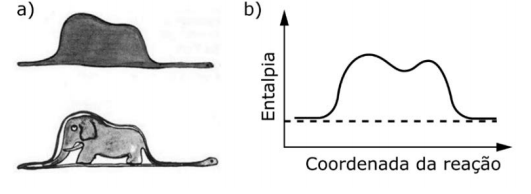
\includegraphics[width=.9\linewidth]{Fisico_Quimica/Termoquimica/figurab.jpg}
\end{center}


\begin{choice}
\choice Praticamente nula, com a formação de dois produtos.
\choice Altamente exotérmica, com a formação de dois produtos.
\choice Altamente exotérmica, mas nada se poderia afirmar sobre a quantidade de espécies no produto.
\choice Praticamente nula, mas nada se poderia afirmar sobre a quantidade de espécies no produto. 
\choice Nenhuma das alternativas.
\end{choice}
\end{exercise}
\begin{solution}
D
\end{solution}





\collectexercisesstop{TermoquimicaI}




\printrandomexercises[collection=LigacaoQuimica]{2}
\printrandomexercises[collection=TeoriaAtomica]{2}
\printrandomexercises[collection=PilhasI]{3}
\printrandomexercises[collection=TermoquimicaI]{3}
\end{document}
